\chapter{Tactics}
\begin{quotation}
\textit{Strategy without tactics is the slowest route to victory. Tactics without strategy is the noise before defeat.}\\
\begin{flushright}Sun Tzu (The Art of War, 476-221 BC)\end{flushright}
\end{quotation}

%%% Beyond the age of information is the age of choices.
%%% -- Charles Eames

%%% Correlation doesn't imply causation, but it does waggle its eyebrows suggestively and gesture furtively while mouthing 'look over there'.
%%% -- Randall Munroe

%%% We learn about who someone is by the choices they make when the choice isn't obvious.
%%% -- Ben Casnocha

%%% Probability theory can tell us how our hypothesis fares relative to the alternatives that we have specified; it does not have the creative imagination to invent new hypotheses for us.
%%% -- E.T. Jaynes, Probability Theory

%%% "Very recently - in just the last few decades - the human species has acquired a great deal of new knowledge about human rationality. The most salient example would be the heuristics and biases program in experimental psychology. There is also the Bayesian systematization of probability theory and statistics; evolutionary psychology; social psychology. Experimental investigations of empirical human psychology; and theoretical probability theory to interpret what our experiments tell us; and evolutionary theory to explain the conclusions. These fields give us new focusing lenses through which to view the landscape of our own minds. With their aid, we may be able to see more clearly the muscles of our brains, the fingers of thought as they move. We have a shared vocabulary in which to describe problems and solutions. Humanity may finally be ready to synthesize the martial art of mind: to refine, share, systematize, and pass on techniques of personal rationality."
%%% -- Eliezer Yudkowsky

%%% Your calendar never lies. All we have is our time. The way we spend our time is our priorities, is our "strategy." Your calendar knows what you really care about. Do you?
%%% -- Tom Peters, HT Ben Casnocha

%%% When things are hard to understand, people who suspect they're nonsense generally keep quiet.
%%% -- Paul Graham

%%% "Don't worry about what anybody else is going to do.do The best way to predict the future is to invent it."
%%% - Alan Kay

%%% "The imagination of nature is far, far greater than the imagination of man."
%%% - Richard Feynman

%%% “SUCCESS: to laugh often and much; to win the respect of intelligent people and the affection of children; to earn the appreciation of honest critics and endure the betrayal of false friends; to appreciate beauty, to find the best in others; to leave the world a bit better, whether by a healthy child, a garden patch or a redeemed social condition ; to know even one life has breathed easier because you have lived. This is to have succeeded.” Emerson

\lettrine{I}{ntro}

\chaptertoc

\begin{itemize}
\item Problem: make the most efficient tactical decisions (attacks and defenses) in the absolute (knowing everything: armies positions, players intentions, effects of each possible actions).
\item Problem that we solve: make the most efficient tactical decisions (in average) knowing what we saw from the opponent and our model of the game. 
\item Type: prediction is problem of \textit{inference from partial observations}; adaptation given what we know is a problem of \textit{decision-making under uncertainty}.
\item Complexity: EXPTIME-complete (as for Chess and Go \citep{Robson83}). Our solutions are real-time on a laptop.
\end{itemize}

%We believe video game AI is central to new, fun, re-playable gameplays, being them multi-player or not. Cooperative (player versus AI) games are enjoying a new boom, recent RTS games delegate more micro-management to the AI as ever, and ever more realistic first-person shooters (FPS) immersion hardly cope with scripted (unsurprising) non-playing characters (NPC). 
In their study on human like characteristics in RTS games, Hagelb\"{a}ck and Johansson \cite{HagelbackCIG10} found out that ``tactics was one of the most successful indicators of whether the player was human or not''. 
%No current non-cheating AI consistently beats good human players in RTS (aim cheating is harder to define for FPS games), nor are fun to play many games against. Finally, multi-player game AI research is in between real-world robotics (the world is simulated but not the players) and more theoretical AI and can benefit both fields.

\begin{figure}[!ht]
\begin{center}
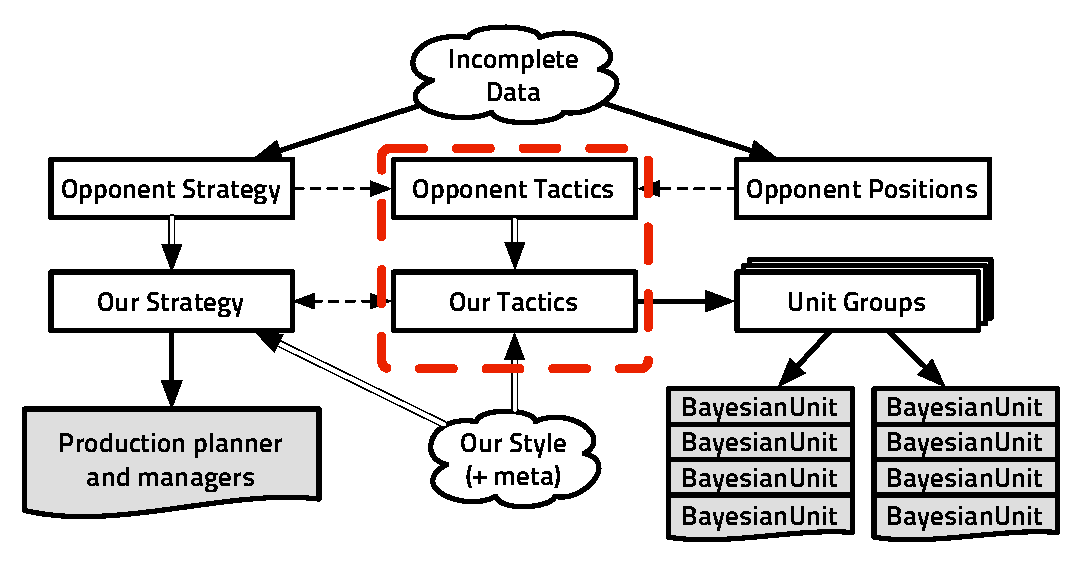
\includegraphics[width=13cm]{images/starcraft_bbq_concept_TACTICS.pdf}
\end{center}
\label{fig:conceptTACTICS}
\caption{Information-centric view of the architecture of the bot, the part concerning this chapter is in the dotted rectangle}
\end{figure}
\begin{itemize}
\item Problem: choose which tactical actions/goals to persue, peform the action
\item Complexity: incompleteness/uncertainty problem, lot of low level information to handle, w.r.t. full and higher level information, simple.
\item State of the art: \citep{SORTS, Weber2010cr, UCT, CadenaG11}
\item Our take: low level heuristics that we learn to adapt to
\item Results: XXX
\item Conclusion and perspectives: still enabled for meta-game, and even in-game, adaptation. Could learn the action sequences of tactics from replays ($\approx$HMM).
\end{itemize}

\section{What are Tactics?}
In this part, we focus on tactics, in between strategy (high-level) and micro-management (lower-level), as seen in Fig.~\ref{fig:sc_abstraction_tactics}. We propose a model which can either predict enemy attacks or give us a distribution on where and how to attack the opponent. Information from the higher-level strategy constrains what types of attacks are possible. As shown in Fig.~\ref{fig:sc_abstraction_tactics}, information from units positions (or possibly an enemy units particle filter as in \cite{weber2011aiide}) constrains where the armies can possibly be in the future. In the context of our StarCraft bot, once we have a decision: we generate a goal (attack order) passed to units groups (see Fig.\ref{fig:conceptTACTICS}). A Bayesian model for micro-management \cite{SYNNAEVE:Micro}, in which units are attracted or repulsed by dynamic (goal, units, damages) and static (terrain) influence maps, actually moves the units in StarCraft. Other previous works on strategy prediction \cite{SYNNAEVE:StratPred,SYNNAEVE:OpeningPred} allows us to infer the enemy tech tree and strategies from incomplete information (due to the fog of war).


Units have different abilities, which leads to different possible tactics. Each faction has invisible (temporarily or permanently) units, flying transport units, flying attack units and ground units. Some units can only attack ground or air units, some others have splash damage attacks, immobilizing or illusion abilities. Fast and mobile units are not cost-effective in head-to-head fights against slower bulky units. We used the gamers' vocabulary to qualify different types of tactics: \textit{ground} attacks (raids or pushes) are the most normal kind of attacks, carried by basic units which cannot fly. Then comes \textit{air} attacks (air raids), which use flying units mobility to quickly deal damage to undefended spots. \textit{Invisible} attacks exploit the weaknesses (being them positional or technological) in detectors of the enemy to deal damage without retaliation. Finally, \textit{drops} are attacks using ground units transported by air, combining flying units mobility with cost-effectiveness of ground units, at the expense of vulnerability during transit.


\section{Related Works}
Aha et al. \cite{LTW} used case-based reasoning (CBR) to perform dynamic tactical plan retrieval (matching) extracted from domain knowledge in Wargus. Onta\~{n}\'{o} et al. \cite{Ontanon07} based their real-time case-based planning (CBP) system on a plan dependency graph which is learned from human demonstration in Wargus. A case based behavior generator spawn missing goals which are missing from the current state and plan according to the recognized state. In \cite{PlanRetrieval,meta-rts}, they used a knowledge-based approach to perform situation assessment to use the right plan, performing runtime adaptation by monitoring its performance. Sharma et al. \cite{CBR-RL} combined CBR and reinforcement learning to enable reuse of tactical plan components. Cadena and Garrido \cite{CadenaG11} used fuzzy CBR (fuzzy case matching) for strategic and tactical planning. Chung et al. \cite{Chung05} adapted Monte-Carlo tree search (MCTS) to planning in RTS games and applied it to a capture-the-flag mod of Open RTS. Balla and Fern \cite{Balla_uctfor} applied upper confidence bounds on trees (UCT: a MCTS algorithm) to tactical assault planning in Wargus. 

In Starcraft, Weber et al. \cite{Weber2010cr,WeberCIG10} produced tactical goals through reactive planning and goal-driven autonomy, finding the more relevant goal(s) to follow in unforeseen situations. Kabanza et al. \cite{OBRecog} performs plan and intent recognition to find tactical opportunities. %\cite{Churchill2011} used abstractions and heuristics to produce a real-time build-order planner.
On spatial and temporal reasoning, Forbus et al. \cite{Forbus2002} presented a tactical qualitative description of terrain for wargames through geometric and pathfinding analysis. Perkins \cite{Perkins2010} automatically extracted choke points and regions of StarCraft maps from a pruned Voronoi diagram, which we used for our regions representations. Wintermute et al. \cite{SORTS} used a cognitive approach mimicking human attention for tactics and units control. Ponsen et al. \cite{PonsenMSA06} developed an evolutionary state-based tactics generator for Wargus. %On influence maps, \cite{teamCompositionRTS} studied team composition and maneuvering by learning a self-organizing map, while \cite{HagelbackJ08} presented a multi-agent potential field based bot .....
Finally, Avery et al. \cite{Avery09} and Smith et al. \cite{SmithCIG10} co-evolved influence map trees for spatial (tactical) reasoning in RTS games. 

Our approach (and bot architecture, depicted in Fig.~\ref{fig:conceptTACTICS}) can be seen as goal-driven autonomy \cite{Weber2010cr} dealing with multi-level reasoning by passing distributions (without any assumption about how they were obtained) on the module input. Using distributions as messages between specialized modules makes dealing with uncertainty first class, this way a given model do not care if the uncertainty comes from incompleteness in the data, a complex and biased heuristic, or another probabilistic model. We then take a decision by sampling or taking the most probable value in the output distribution. Another particularity of our model is that it allows for prediction of the enemy tactics using the same model with different inputs. Finally, our approach is not exclusive to most of the techniques presented above, and it could be interesting to combine it with UCT \cite{Balla_uctfor} and more complex/precise tactics generated through planning.

\section{A Bayesian Tactical Model}
\subsection{Dataset}
% PvP 1336, PvT 7225, PvZ 6082, TvT 1384, TvZ 6322, ZvZ 598
We downloaded more than 25,000 replays to keep 22,947 uncorrupted, 1v1 replays of very high level StarCraft games (pro-gamers leagues and international tournaments) from specialized websites\footnote{\url{http://www.teamliquid.net}}\footnote{\url{http://www.gosugamers.net}}\footnote{\url{http://www.iccup.com}}, we then ran them using BWAPI\footnote{\url{http://code.google.com/p/bwapi/}} and dumped units positions, pathfinding and regions, resources, orders, vision events, for attacks (we trigger an attack tracking heuristic when one unit dies and there are at least two military units around): types, positions, outcomes. Basically, every BWAPI event was recorded, the dataset and its source code are freely available\footnote{\url{http://snippyhollow.github.com/bwrepdump/}}. 

We used two kinds of regions: BroodWar Terrain Analyser (BWTA) regions and choke-dependent (choke-centered) regions. BWTA regions are obtained from a pruned Voronoi diagram on walkable terrain \cite{Perkins2010} and gives regions for which chokes are the boundaries. As battles often happens at chokes, choke-dependent regions are created by doing an additional (distance limited) Voronoi tesselation spawned at chokes, its regions set is $(regions \setminus chokes) \cup chokes$. Results for choke-dependent regions are not fully detailed.

\subsection{Tactical Model}
The idea is to have (most probably biased) lower-level heuristics from units observations which produce information exploitable at the tactical level, and take some advantage of strategic inference too. The advantages are that 1) learning will de-skew the model output from biased heuristic inputs 2) the model is agnostic to where input variables' values come from 3) the updating process is the same for supervised learning and for reinforcement learning. 

We note $s^{a|d}_{unit\ type}(r)$ for the balanced score of units from attacker or defender ($^{a|d}$) of a given type in region $r$. The balanced score of units is just the sum of units multiplied by each unit score ($= minerals\_value + \frac{4}{3}gas\_value + 50supply\_value$). The heuristics we used in our benchmarks (which we could change) are: 
%\begin{itemize}
$$economical\_score^d(r) = \frac{s^d_{workers}(r)}{\sum_r s^d_{workers}(r)}$$
$$tactical\_score^d(r) = \sum_{i \in regions} s^d_{army}(i) \times dist(i,r)^{-1.5}$$
We used $^{-1.5}$ such that the tactical value of a region in between two halves of an army, each at distance 2, would be higher than the tactical value of a region at distance 4 of the full (same) army. For flying units, \textit{dist} is the Euclidean distance, while for ground units it takes pathfinding into account.
$$ground\_defense^d(r) = \frac{s^d_{can\_attack\_ground}(r)}{s^a_{ground\_units}(r)}$$
$$air\_defense^d(r) = \frac{s^d_{can\_attack\_air}(r)}{s^a_{air\_units}(r)}$$
$$invis\_defense^d(r) = number^d_{detectors}$$
%\end{itemize}

We preferred to discretize continuous values to enable quick complete computations. An other strategy would keep more values and use Monte Carlo sampling for computation. We think that discretization is not a concern because 1) heuristics are simple and biased already 2) we often reason about imperfect information and this uncertainty tops discretization fittings.
\subsubsection{Variables}
With $n$ regions, we have: 
\begin{itemize}
    \item $A_{1:n} \in \{true,false\}$, $A_i$: attack in region $i$ or not?
    \item $E_{1:n} \in \{no, low, high\}$, $E_i$ is the discretized economical value of the region $i$ for the defender. We choose 3 values: \textit{no} workers in the regions, \textit{low}: a small amount of workers (less than half the total) and \textit{high}: more than half the total of workers in this region $i$.
    \item $T_{1:n} \in dicrete\ levels$, $T_i$ is the tactical value of the region $i$ for the defender, see above for an explanation of the heuristic. Basically, $T$ is proportional to the proximity to the defender's army. In benchmarks, discretization steps are $0,0.05,0.1,0.2,0.4,0.8$ ($log_2$ scale).
    \item $TA_{1:n} \in dicrete\ levels$, $TA_i$ is the tactical value of the region $i$ for the attacker (see above).
    \item $B_{1:n} \in \{true, false\}$, $B_i$ tells if the region belongs (or not) to the defender. $\PP(B_i=true)=1$ if the defender has a base in region $i$ and $\PP(B_i=false)=1$ if the attacker has one. Influence zones of the defender can be measured (with uncertainty) by $\PP(B_i=true) \geq 0.5$ and vice versa.
    \item $H_{1:n} \in \{ground, air, invisible, drop\}$, $H_i$: in predictive mode: how we will be attacked, in decision-making: how to attack, in region $i$.
    \item $GD_{1:n} \in \{no, low, med, high\}$: ground defense (relative to the attacker power) in region $i$, result from a heuristic. \textit{no} defense if the defender's army is $\geq 1/10th$ of the attacker's, \textit{low} defense above that and under half the attacker's army, \textit{medium} defense above that and under comparable sizes, \textit{high} if the defender's army is bigger than the attacker.
    \item $AD_{1:n} \in \{no, low, med, high\}$: same for air defense.
    \item $ID_{1:n} \in \{no\ detector, one\ detector, several\}$: invisible defense, equating to numbers of detectors.
    \item $TT \in [\emptyset, building_1, building_2, building_1\wedge building_2, techtrees, \dots]$: all the possible technological trees for the given race. For instance $\{pylon, gate\}$ and $\{pylon, gate, core\}$ are two different $T$ech $T$rees.
    \item $P \in \begin{small}\{ground, ground\wedge air, ground\wedge invis, ground\wedge air\wedge invis, ground\wedge drop, ground\wedge air\wedge drop, ground\wedge invis\wedge drop, ground\wedge air\wedge invis\wedge drop\}\end{small}$: possible types of attacks, directly mapped from $TT$ information. In prediction, with this variable, we make use of what we can infer on the opponent's strategy \cite{SYNNAEVE:OpeningPred,SYNNAEVE:StratPred}, in decision-making, we know our own possibilities (we know our tech tree as well as the units we own).
    %\item
\end{itemize}
Finally, for some variables, we take uncertainty into account with ``soft evidences'': for instance for a region in which no player has a base, we have a soft evidence that it belongs more probably to the player established closer. In this case, for a given region, we introduce the soft evidence variable(s) $B'$ and the coherence variable $\lambda_B$ and impose $\PP(\lambda_B=1|B,B')\ iff\ B=B'$, while $\PP(\lambda_B|B,B').\PP(B')$ is a new factor in the joint distribution. This allows to sum over $\PP(B')$ distribution (soft evidence). 

\subsubsection{Decomposition}
The joint distribution of our model contains soft evidence variables for all input family variables ($E,T,TA,B,GD,AD,ID,P$) to be as general as possible, \textit{i.e.} to be able to cope with all possible uncertainty (from incomplete information) that may come up in a game. To avoid being too verbose, we explain the decomposition only with the soft evidence for the family of variables $B$, the principle holds for all other soft evidences. For the $n$ considered regions, we have:
\begin{eqnarray*}
    & & \PP(A_{1:n}, E_{1:n}, T_{1:n}, TA_{1:n}, B_{1:n}, B'_{1:n}, \lambda_{B,1:n}, \\
& & H_{1:n}, GD_{1:n}, AD_{1:n}, ID_{1:n}, P, TT) \\
    & = & \prod_{i=1}^n [\PP(A_i).\PP(E_i,T_i,TA_i,B_i|A_i).\ \ \ \ \ \ \ \ \ \ \ \ \ \mathrm{(1)}\\
& & \PP(\lambda_{B,i} | B_{1:n},B'_{1:n}).\PP(B'_{1:n}). \\
& & \PP(AD_i,GD_i,ID_i|H_i).\PP(H_i|P)].\PP(P|TT).\PP(TT)
\end{eqnarray*}

\subsubsection{Forms and Learning}
We will explain the forms for a given/fixed $i$ region number:
\begin{itemize}
\item $\PP(A)$ is the prior on the fact that the player attacks in this region, in our evaluation we set it to $n_{battles}/(n_{battles}+n_{not\ battles})$. In a given match it should be initialized to uniform and progressively learn the preferred attack regions of the opponent for predictions, learn the regions in which our attacks fail or succeed for decision-making.
\item $\PP(E,T,TA,B|A)$ is a covariance table of the economical, tactical (both for the defender and the attacker), belonging scores where an attacks happen. We just use Laplace succession law (``add one'' smoothing) \cite{Jaynes} and count the co-occurrences, thus almost performing maximum likelihood learning of the table.
\item $\PP(\lambda_{B}|B,B') = 1.0\ iff\ B=B'$ is just a coherence constraint.
\item $\PP(AD,GD,ID|H)$ is a covariance table of the air, ground, invisible defense values depending on how the attack happens. As for $\PP(E,T,TA,B|A)$, we use a Laplace's law of succession to learn it.
\item $\PP(H|P)$ is the distribution on how the attack happens depending on what is possible. Trivially $\PP(H=ground|P=ground)=1.0$, for more complex possibilities we have different maximum likelihood multinomial distributions on $H$ values depending on $P$.
\item $\PP(P|TT)$ is the direct mapping of what the tech tree allows as possible attack types: $\PP(P=p|TT)=1$ is a function of $TT$ (all $\PP(P\neq p|TT)=0$).
\item $\PP(TT)$: if we are sure of the tech tree (prediction without fog of war, or in decision-making mode), $\PP(TT=k)=1$ and $\PP(TT\neq k)=0$; otherwise, it allows us to take uncertainty about the opponent's tech tree and balance $\PP(P|TT)$. We obtain a distribution on what is possible ($\PP(P)$) for the opponent's attack types.
\end{itemize}
There are two approaches to fill up these probability tables, either by observing games (supervised learning), as we did in the evaluation section, or by acting (reinforcement learning). %We first learned all the parameters from observations on the dataset. 
In match situation against a given opponent, for inputs that we can unequivocally attribute to their intention (style and general strategy), we also refine these probability tables (with Laplace's rule of succession). To keep things simple, we just refine $\sum_{E,T,TA}\PP(E,T,TA,B|A)$ corresponding to their aggressiveness (aggro) or our successes and failures, and equivalently for $\PP(H|P)$. Indeed, if we sum over $E$, $T$ and $TA$, we consider the inclination of our opponent to venture into enemy territory or the interest that we have to do so by counting our successes with aggressive or defensive parameters. In $\PP(H|P)$, we are learning the opponent's inclination for particular types of tactics according to what is available to their, or for us the effectiveness of our attack types choices.

The model is highly modular, and some parts are more important than others. We can separate three main parts: $\PP(E,T,TA,B|A)$, $\PP(AD,GD,ID|H)$ and $\PP(H|P)$. In prediction, $\PP(E,T,TA,B|A)$ uses the inferred (uncertain) economic ($E$), tactical ($T$) and belonging ($B$) scores of the opponent while knowing our own tactical position fully ($TA$). In decision-making, we know $E,T,B$ (for us) and estimate $TA$. In our prediction benchmarks, $\PP(AD,GD,ID|H)$ has the lesser impact on the results of the three main parts, either because the uncertainty from the attacker on $AD,GD,ID$ is too high or because our heuristics are too simple, though it still contributes positively to the score. In decision-making, it allows for reinforcement learning to have pivoting tuple values for $AD,GD,ID$ at which to switch attack types. In prediction, $\PP(H|P)$ is used to take $\PP(TT)$ (coming from strategy prediction \cite{SYNNAEVE:StratPred}) into account and constraints $H$ to what is possible. For the use of $\PP(H|P).\PP(P|TT).\PP(TT)$ in decision-making, see the Results sections.

\subsubsection{Questions}
For a given region $i$, we can ask the probability to attack here,
\begin{equation*}
\PP(A_i=a_i|e_i,t_i,ta_i,\lambda_{B,i}=1)
\end{equation*}
\vspace{-0.2cm}
\begin{small}
\begin{equation*}
= \frac{\sum_{B_i,B_i'}\PP(e_i,t_i,ta_i,B_i|a_i).\PP(a_i).\PP(B_i').P(\lambda_{B,i}|B_i,B_i')}{\sum_{A_i,B_i,B_i'}\PP(e_i,t_i,ta_i,B_i|A_i).\PP(A_i).\PP(B_i').\PP(\lambda_{B,i}|B_i,B_i')}
\end{equation*}
\end{small}
\vspace{-0.2cm}
\begin{equation*}
\propto \sum_{B_i,B_i'}\PP(e_i,t_i,ta_i,B_i|a_i).\PP(a_i).\PP(B_i').\PP(\lambda_{B,i}|B_i,B_i')
\end{equation*}
and the mean by which we should attack,
\begin{eqnarray*}
& & \PP(H_i=h_i|ad_i,gd_i,id_i) \\
& \propto & \sum_{TT,P}[\PP(ad_i,gd_i,id_i|h_i).\PP(h_i|P).\PP(P|TT).\PP(TT)]
\end{eqnarray*}
For clarity, we omitted some variables couples on which we have to sum (to take uncertainty into account) as for $B$ (and $B'$) above. We always sum over estimated, inferred variables, while we know the one we observe fully. In prediction mode, we sum oover $TA,B,TT,P$; in decision-making, we sum over $E,T,B,AD,GD,ID$. 
The complete question that we ask our model is $\PP(A,H|FullyObserved)$. The maximum of $\PP(A,H)$ may not be the same as the maximum of $\PP(A)$ or $\PP(H)$, for instance think of a very important economic zone that is very well defended, it may be the maximum of $\PP(A)$, but not once we take $\PP(H)$ into account. Inversely, some regions are not defended against anything at all but present little or no interest. Our joint distribution (1) can be rewritten: $\PP(Searched,FullyObserved,Estimated)$, so we ask:
\begin{eqnarray*}
& & \PP(A_{1:n},H_{1:n}|FullyObserved) \ \ \ \ \ \ \ \ \ \ \ \ \ \ \ \ \ \  \mathrm(2) \\
& \propto & \sum_{Estimated}\PP(A_{1:n},H_{1:n},Estimated,FullyObserved)
\end{eqnarray*}


\section{Results on StarCraft}

\subsection{Learning}
To measure fairly the prediction performance of such a model, we applied ``leave-100-out'' cross-validation from our dataset: as we had many games (see Table.~\ref{tab:all_results}), we set aside 100 games of each match-up for testing (with more than 1 battle per match: rather $\approx 15$ battles/match) and train our model on the rest. We write match-ups XvY with X and Y the first letters of the factions involved (Protoss, Terran, Zerg). Note that mirror match-ups (PvP, TvT, ZvZ) have less games but twice as much attacks from a given faction. Learning was performed as explained in III.B.3: for each battle in $r$ we had one observation for: $\PP(e_r,t_r,ta_r,b_r|A=true)$, and $\#regions-1$ observations for the $i$ regions which were not attacked: $\PP(e_{i \neq r},t_{i \neq r}, ta_{i \neq r}, b_{i \neq r}|A=false)$. For each battle of type $t$ we had one observation for $P(ad,gd,id|H=t)$ and $P(H=t|p)$. By learning with a Laplace's law of succession \cite{Jaynes}, we allow for unseen event to have a non-null probability.

An exhaustive presentation of the learned tables is out of the scope of this paper, but we displayed interesting cases in which the learned probability tables meet concur with human expertise in Figures~\ref{fig:P_H_AD},\ref{fig:PossibleP},\ref{fig:Where3D}. In Fig.~\ref{fig:P_H_AD}, we see that air raids/attacks are quite risk averse and it is two times more likely to attack a region with less than 1/10th of the flying force in anti-aircraft warfare than to attack a region with up to one half of our force. We can also notice than drops are to be preferred either when it is safe to land (no anti-aircraft defense) or when there is a large defense (harassment tactics). In Fig.~\ref{fig:PossibleP} we can see that, in general, there are as much ground attacks at the sum of other types. The two top graphs show cases in which the tech of the attacker was very specialized, and, in such cases, the specificity seems to be used. In particular, the top right graphic may be corresponding to a ``fast Dark Templars rush''. Finally, Fig.~\ref{fig:Where3D} shows the transition between two types of encounters: tactics aimed at engaging the enemy army (a higher $T$ value entails a higher $\PP(A)$) and tactics aimed at damaging the enemy economy (at high $E$, we look for opportunities to attack with a small army where $T$ is lower).

\begin{figure}[htp]
\centerline{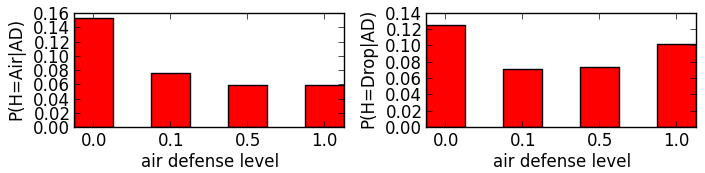
\includegraphics[width=11cm]{images/Terran_Prob_H_knowing_AD.png}}
%\vspace{-0.3cm}
\caption{$\PP(H=air)$ and $\PP(H=drop)$ for varying values of $AD$ (summed on other variables), for Terran in TvP.}
\label{fig:P_H_AD}
%\vspace{-0.5cm}
\end{figure}

\begin{figure}[htp]
\centerline{\includegraphics[width=11cm]{images/PossibleP.png}}
%\vspace{-0.3cm}
\caption{$\PP(H|P)$ for varying values $H$ and for different values of $P$ (derived from inferred $TT$), for Protoss in PvT.}
\label{fig:PossibleP}
%\vspace{-0.5cm}
\end{figure}

\begin{figure}[htp]
\centerline{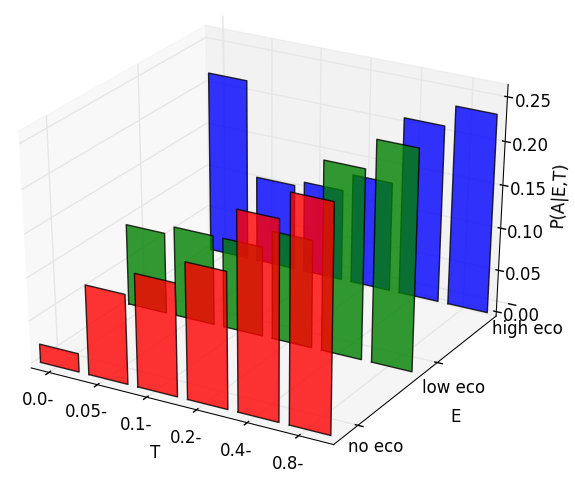
\includegraphics[width=9cm]{images/where3D_EI_TI_RegT.png}}
%\vspace{-0.3cm}
\caption{$\PP(A)$ for varying values of $E$ and $T$, summed on the other variables, for Terran in TvT.}
\label{fig:Where3D}
%\vspace{-0.5cm}
\end{figure}

\subsection{Prediction Performance}
We learned and tested one model for each race and each match-up. As we want to predict \textit{where} ($\PP(A_{1:n})$) and \textit{how} ($\PP(H_{battle})$) the next attack will happen to us, we used inferred enemy $TT$ (to produce $P$) and $TA$, our scores being fully known: $E$, $T$, $B$, $ID$. We consider $GD$, $AD$ to be fully known even though they depend on the attacker force, we should have some uncertainty on them, but we tested that they accounted (being known instead of fully unknown) for 1 to 2\% of $\PP(H)$ accuracy (in prediction) once $P$ was known. We should point that pro-gamers scout very well and so it allows for a highly accurate $TT$ estimation with \cite{SYNNAEVE:StratPred}. Training requires to recreate battle states (all units positions) and count parameters for 5,000 to 30,000 battles. Once that is done, inference is very quick: a look-up in a probability table for known values and $\#F$ look-ups for free variables $F$ on which we sum. We chose to try and predict the next battle 30 seconds before it happens, 30 seconds being an approximation of the time needed to go from the middle of a map (where the entropy on ``next battle position'' is maximum) to any region by ground, so that the prediction is useful for the defender (they can position their army).

The model code\footnote{\url{https://github.com/SnippyHolloW/AnalyzeBWData}} (for learning and testing) as well as the datasets (see above) are freely avaible. Raw results of predictions of positions and types of attacks 30 seconds before they happen are presented in Table.~\ref{tab:all_results}: for instance the bold number (38.0) corresponds to the percentage of good positions (regions) predictions (30 sec before event) which were ranked 1st in the probabilities on $A_{1:n}$ for Protoss attacks against Terran (PvT). The measures on \textit{where} corresponds to the percentage of good prediction and the mean probability for given ranks in $\PP(A_{1:n})$ (to give a sense of the shape of the distribution). As the most probable The measures on \textit{how} corresponds to the percentage of good predictions for the most probable $\PP(H_{battle})$ and the number of such battles seen in the test set for given attack types. We particularly predict well ground attacks (trivial in the early game, less in the end game) and, interestingly, Terran and Zerg drop attacks. The \textit{where \& how} row corresponds to the percentage of good predictions for the maximal probability in the joint $\PP(A_{1:n},H_{1:n})$: considering only the most probable attack (more information is in the rest of the distribution, as shown for \textit{where}!) according to our model, we can predict \textit{where} \textbf{and} \textit{how} an attack will occur in the next 30 seconds $\approx$ 1/4th of the time. Finally, note that scores are not ridiculous 60 seconds before the attack neither (obviously, $TT$, and thus $P$, are not so different, nor are $B$ and $E$): PvT \textit{where} top 4 ranks are 35.6, 8.5, 7.7, 7.0\% good versus 38.0, 16.3, 8.9, 6.7\% 30 seconds before; \textit{how} total precision 60 seconds before is 70.0\% vs. 72.4\%, \textit{where \& how} maximum probability precision is 19.9\% vs. 23\%.

\setlength{\tabcolsep}{4.69pt}
\begin{table*}[ht]
\caption{Results summary for multiple metrics at 30 seconds before attack. The number in bold (38.0) is read as ``38\% of the time, the region $i$ with probability of rank 1 in $\PP(A_i)$ is the one in which the attack happened 30 seconds later''.}
\begin{center}
%\begin{small}
\begin{footnotesize}
\begin{tabular}{|cc|cc|cc|cc|cc|cc|cc|cc|cc|cc|}
\hline
\multicolumn{2}{|c|}{\%: good predictions} & \multicolumn{6}{||c|}{Protoss} & \multicolumn{6}{|c|}{Terran} & \multicolumn{6}{|c|}{Zerg} \\
\multicolumn{2}{|c|}{Pr: mean probability} & \multicolumn{2}{||c|}{P} & \multicolumn{2}{|c|}{T} & \multicolumn{2}{|c|}{Z} & \multicolumn{2}{|c|}{P} & \multicolumn{2}{|c|}{T} & \multicolumn{2}{|c|}{Z} & \multicolumn{2}{|c|}{P} & \multicolumn{2}{|c|}{T} & \multicolumn{2}{|c|}{Z} \\
\hline
% PvP 1336, PvT 7225, PvZ 6082, TvT 1384, TvZ 6322, ZvZ 598
\multicolumn{2}{|c|}{total \# games} & \multicolumn{2}{|c|}{1336} & \multicolumn{2}{|c|}{7225}& \multicolumn{2}{|c|}{6082}& \multicolumn{2}{|c|}{7225}& \multicolumn{2}{|c|}{1384}& \multicolumn{2}{|c|}{6322}& \multicolumn{2}{|c|}{6082}& \multicolumn{2}{|c|}{6322}& \multicolumn{2}{|c|}{598}\\
\hline
measure & rank & \% & Pr & \% & Pr & \% & Pr & \% & Pr & \% & Pr& \% & Pr& \% & Pr& \% & Pr& \% & Pr  \\
\hline
 & 1 & 40.9 & .334 & \textbf{38.0} & .329 & 34.5 & .304 & 35.3 & .299 & 34.4 & .295 & 39.0 & 0.358 & 32.8 & .31 & 39.8 & .331 & 37.2 & .324 \\
\multirow{3}{3mm}{\begin{sideways}\parbox{3mm}{\begin{small}where\end{small}}\end{sideways}}
 & 2 & 14.6 & .157 & 16.3 & .149 & 13.0 & .152 & 14.3 & .148 & 14.7 & .0147 & 17.8 & .174 & 15.4 & .166 & 16.6 & .148 & 16.9 & .157 \\
 & 3 & 7.8 & .089 & 8.9 & .085 & 6.9 & .092 & 9.8 & .09 & 8.4 & .087 & 10.0 & .096 & 11.3 & .099 & 7.6 & .084 & 10.7 & .100 \\
 & 4 & 7.6 & .062 & 6.7 & .059 & 7.9 & .064 & 8.6 & .071 & 6.9 & .063 & 7.0 & .062 & 8.9 & .07 & 7.7 & .064 & 8.6 & .07 \\
%\multicolumn{2}{|c|}{distance best} & \multicolumn{2}{|c|}{32} &\\
\hline
measure & type & \% & N & \% & N & \% & N & \% & N & \% & N & \% & N & \% & N & \% & N & \% & N \\
\hline
 & G & 97.5 & 1016 & 98.1 & 1458 & 98.4 & 568 & 100 & 691 & 99.9 & 3218 & 76.7 & 695 & 86.6 & 612 & 99.8 & 567 & 67.2 & 607 \\
\multirow{3}{3mm}{\begin{sideways}\parbox{3mm}{\begin{small}how\end{small}}\end{sideways}}
 & A & 44.4 & 81 & 34.5 & 415 & 46.8 & 190 & 40 & 5 & 13.3 & 444 & 47.1 & 402 & 14.2 & 155 & 15.8 & 19 & 74.2 & 586 \\
 & I & 22.7 & 225 & 49.6 & 337 & 12.9 & 132 & NA & NA & NA & NA & 36.8 & 326 & 32.6 & 227 & NA & NA & NA & NA \\
 & D & 55.9 & 340 & 42.2 & 464 & 45.2 & 93 & 93.5 & 107 & 86 & 1183 & 62.8 & 739 & 67.7 & 535 & 81.4 & 86 & 63.6 & 588 \\
\multicolumn{2}{|c|}{total} & 76.3 & 1662 & 72.4 & 2674 & 71.9 & 983 & 98.4 & 806 & 88.5 & 4850 & 60.4 & 2162 & 64.6 & 1529 & 94.7 & 674 & 67.6 & 1802 \\
\hline
\multicolumn{2}{|c|}{where \& how (\%)} & \multicolumn{2}{|c|}{32.8} & \multicolumn{2}{|c|}{23}& \multicolumn{2}{|c|}{23.8}& \multicolumn{2}{|c|}{27.1}& \multicolumn{2}{|c|}{23.6}& \multicolumn{2}{|c|}{30.2}& \multicolumn{2}{|c|}{23.3}& \multicolumn{2}{|c|}{30.9}& \multicolumn{2}{|c|}{26.4}\\
\hline
\end{tabular}
\label{tab:all_results}
\end{footnotesize}
%\end{small}
\end{center}
\end{table*}

When we are mistaken, the mean ground distance (pathfinding wise) of the most probable predicted region to the good one (where the attack happens) is 1223 pixels (38 build tiles, or 2 screens in StarCraft's resolution), while the mean max distance on the map is 5506 (172 build tiles). Also, the mean number of regions by map is 19, so a random \textit{where} (attack destination) picking policy would have a correctness of 1/19 (5.23\%). For choke-centered regions, the numbers of good \textit{where} predictions are lower (between 24\% and 32\% correct for the most probable) but the mean number of regions by map is 42. For \textit{where \& how}, a random policy would have a precision of 1/(19*4), and even a random policy taking the high frequency of ground attacks into account would at most be $\approx$ 1/(19*2) correct.
Note that our current model consider a uniform prior on regions (no bias towards past battlefields) and that we do not incorporate any derivative of the armies' movements. There is no player modeling at all: learning and fitting the mean player's tactics is not optimal, so we should specialize the probability tables for each player. Also, we use all types of battles in our training and testing. Short experiments showed that if we used only attacks on bases, the probability of good \textit{where} predictions for the maximum of $\PP(A_{1:n})$ goes above 50\% (which is not a surprise, there are far less bases than regions in which attacks happen). To conclude on tactics positions prediction: if we sum the 2 most probable regions for the attack, we are right at least half the time; if we sum the 4 most probable (for our robotic player, it means it prepares against attacks in 4 regions as opposed to 19), we are right \textbf{$\approx$ 70\%} of the time.

Mistakes on the type of the attack are high for invisible attacks: while these tactics can definitely win a game, the counter is strategic (it is to have detectors technology deployed) more than positional. Also, if the maximum of $\PP(H_{battle})$ is wrong, it doesn't mean than $\PP(H_{battle}=good)=0.0$ at all! The result needing improvements the most is for air tactics, because countering them really is positional, see our discussion in the conclusion.
% distances
% mean: 1047 + 1134 + 1266 + 1257 + 1306 + XXX + 1228 + 1067 + 1480
% max: 5494 + 5605 + 5433 + 5558 + 5475 + 5443
% best CDR: 32%, 29%, 24%, 24%, 26%, XXX, 25%, 28%, 29%

\subsection{In Game Decision-Making}
In a StarCraft game, our bot has to make decisions about where and how to attack or defend, it does so by reasoning about opponent's tactics, bases, its priors, and under strategic constraints (Fig.~\ref{bbq_dataflow}). Once a decision is taken, the output of the tactical model is an offensive or defensive goal. There are different military goal types (base defense, ground attacks, air attacks, drops...), and each type of goal has pre-requisites (for instance: a drop goal needs to have the control of a dropship and military units to become active). The spawned goal then autonomously sets objectives for Bayesian units \cite{SYNNAEVE:Micro}, sometimes procedurally creating intermediate objectives or canceling itself in the worst cases. 

The destinations of goals are from $\PP(A)$, while the type of the goal comes from $\PP(H)$. In input, we fully know tactical scores of the regions according to our military units placement $TA$ (we are the attacker), what is possible for us to do $P$ (according to units available) and we estimate $E$, $T$, $B$, $ID$, $GD$, $AD$ from past (partial) observations. Estimating $T$ is the most tricky of all because it may be changing fast, for that we use a units filter which just decays probability mass of seen units. An improvement would be to use a particle filter \cite{weber2011aiide}, with a learned motion model. From the joint (2) $\PP(A_{1:n},H_{1:n}|ta,p,tt)$ may arise a couple $i,H_i$ more probable than the most probables $\PP(A_i)$ and $\PP(H_j)$ taken separately (the case of an heavily defended main base and a small unprotected expand for instance). Fig.~\ref{fig:WhereHow} displays the mean $\PP(A,H)$ for Terran (in TvZ) attacks decision-making for the most 32 probable type/region tactical couples. It is in this kind of landscape (though more steep because Fig.~\ref{fig:WhereHow} is a mean) that we sample (or pick the most probable couple) to take a decision. Also, we may spawn defensive goals countering the attacks that we predict from the opponent.

\begin{figure}[htp]
\centerline{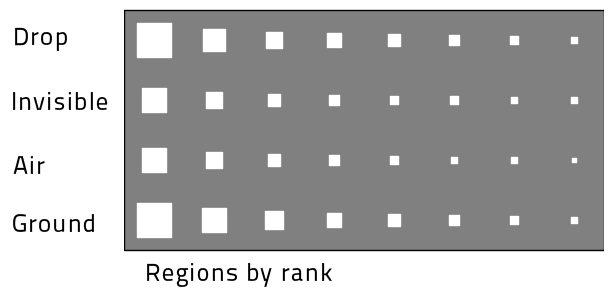
\includegraphics[width=9cm]{images/WhereHow_T_TvZ_light.png}}
%\vspace{-0.3cm}
\caption{Mean $\PP(A,H)$ for all $H$ values and the top 8 $\PP(A_i,H_i)$ values, for Terran in TvZ. The larger the white square area, the higher $\PP(A_i,H_i)$.}
\label{fig:WhereHow}
%\vspace{-0.5cm}
\end{figure}

Finally, we can steer our technological growth towards the opponent's weaknesses. A question that we can ask our model (at time $t$) is $\PP(TT)$, or, in two parts: we first find $i,h_i$ which maximize $\PP(A,H)$ at time $t+1$, and then ask a more directive:
$$\PP(TT|h_i) \propto \sum_{P} \PP(h_i|P).\PP(P|TT).\PP(TT)$$
so that it gives us a distribution on the tech trees ($TT$) needed to be able to perform the wanted attack type. To take a decision on our technology direction, we can consider the distances between our current $tt^t$ and all the probable values of $TT^{t+1}$.

\section{Extensions}
%\subsection{Possible Improvements}
There are three main research directions for possible improvements: improving the underlying heuristics, improving the dynamic of the model and improving the model itself. The heuristics presented here are quite simple but they may be changed, and even removed or added, for another RTS or FPS, or for more performance. In particular, our ``defense against invisible'' heuristic could take detector positioning/coverage into account. Our heuristic on tactical values can also be reworked to take terrain tactical values into account (chokes and elevation in StarCraft). For the estimated position of enemy units, we could use a particle filter \cite{weber2011aiide} with a motion model (at least one for ground units and one for flying units). There is room to improve the dynamics of the model: considering the prior probabilities to attack in regions given past attacks and/or considering evolutions of the $T$,$TA$,$B$,$E$ values (derivatives) in time. The discretizations that we used may show their limits, though if we want to use continuous values, we need to setup a more complicated learning and inference process (MCMC sampling). Finally, one of the strongest assumptions (which is a drawback particularly for prediction) of our model is that the attacking player is always considered to attack in this most probable regions. While this would be true if the model was complete (with finer army positions inputs and a model of what the player thinks), we believe such an assumption of completeness is far fetched. Instead we should express that incompleteness in the model itself and have a ``player decision'' variable $D \sim Multinomial(\PP(A_{1:n},H_{1:n}),player)$.

% We have presented a Bayesian tactical model for RTS AI, which allows both for opposing tactics prediction and autonomous tactical decision-making. Being a probabilistic model, it deals with uncertainty easily, and its design allows easy integration into multi-granularity (multi-scale) AI systems as needed in RTS AI. Without any temporal dynamics, its exact prediction rate of the joint position and tactical type is in [23-32.8]\% (depending on the match-up), and considering the 4 most probable regions it goes up to $\approx$ 70\%. More importantly, it allows for tactical decision-making under (technological) constraints and (state) uncertainty. It can be used in production thanks to its low CPU and memory footprint. The dataset, its documentation\footnote{\url{http://snippyhollow.github.com/bwrepdump/}}, as well as our model implementation\footnote{\url{https://github.com/SnippyHolloW/AnalyzeBWData}} (and other data-exploration tools) are free software and can be found online. We plan to use this model in our StarCraft AI competition entry bot as it gives our bot tactical autonomy and a way to adapt to our opponent.
